\documentclass[main.tex]{subfiles}

\begin{document}

\subsection{Terzo esercizio}

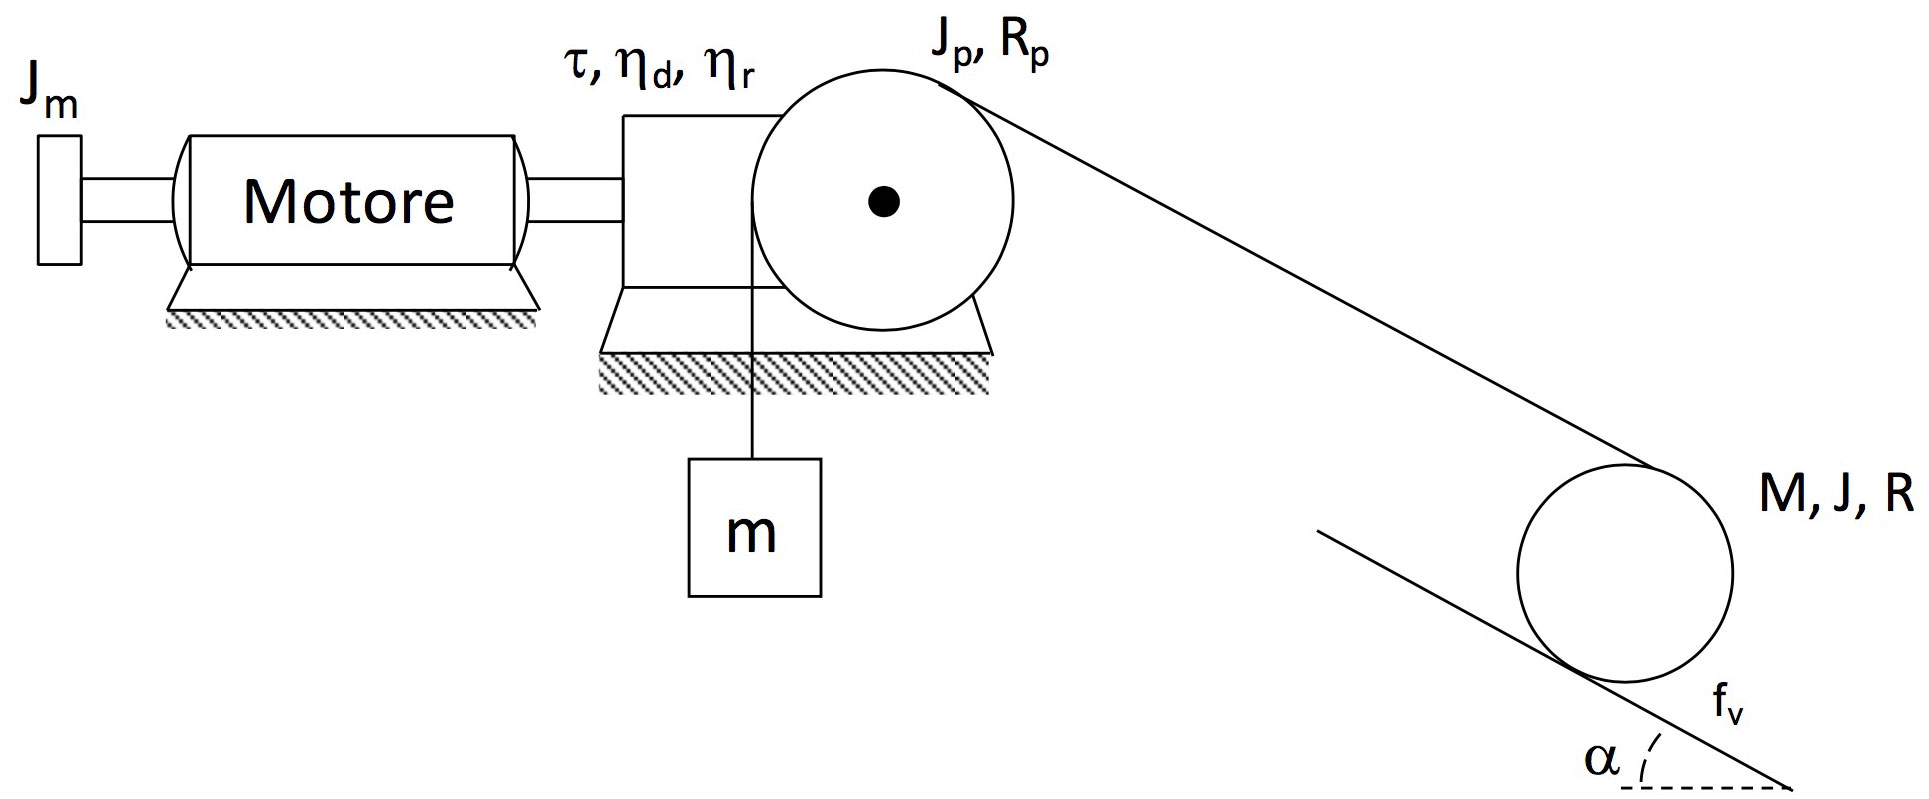
\includegraphics[width=\textwidth]{2015-2906-3.jpg}

\begin{alignat*}{5}
  M=100 kg\quad
  J_m=0.05 kg m^2\quad
  \mu_d =0.9\quad
  \mu_r =0.7\quad
  J=2 kg m^2\quad
  m = 20 kg\quad
\end{alignat*}
\begin{alignat*}{5}
  R=0.5 m \quad
  \alpha =\frac{\pi}{6} \quad
  R_P=0.6 m \quad
  f_v = 0.05\quad
  J_P=5 kg m^2 \quad
  \tau = 1/10 \quad
\end{alignat*}

L’impianto di sollevamento in figura è posizionato nel piano verticale. Un sistema motore- trasmissione solleva, attraverso una puleggia di caratteristiche note (momento d’inerzia baricentrico $J_p$ e raggio $R_p$), un disco (di massa $M$, momento d’inerzia baricentrico $J$ e raggio $R$) che rotola senza strisciare su un piano inclinato di un angolo $\alpha$.

Alla medesima fune, dalla parte opposta al disco, è collegato un contrappeso di massa $m$. Si supponga assenza di strisciamento tra la fune e la puleggia e tra la fune ed il disco.

Sono noti il momento d'inerzia del motore $J_m$ e le caratteristiche della trasmissione (rapporto di trasmissione $\tau$, rendimento in moto diretto $\mu_d$ e rendimento in moto retrogrado $\mu_r$).
\\

Si chiede di calcolare:
\begin{enumerate}
  \item La coppia necessaria per sollevare il disco a regime.
  \item L’accelerazione del disco in salita, applicando una coppia motrice doppia rispetto a quella calcolata al punto 1.
\end{enumerate}

\pagebreak

\subsection{Soluzione terzo esercizio}

\subsubsection{Osservazioni importanti}
\begin{enumerate}
  \item In questo tipo di esercizi è \textbf{necessario} capire in che modo il sistema va a muoversi.
  \item Il sistema è posto sul piano verticale, quindi andranno considerate tutte le forze peso dei vari componenti.
  \item Sul disco agisce una forza di \textit{attrito volvente}.
\end{enumerate}

\subsubsection{Primo punto}
In condizione di regime \textit{la variazione di energia cinetica è nulla}. Per cui vale che:

\[
  W_{motrice} + W_{resistente} + W_{perduta} = \frac{dE_c}{dt} = 0
\]

\begin{figure}[H]
  \begin{align*}
    W_R &= (\text{Forze attrito statico e dinamico})\bullet(\text{Velocità del punto di applicazione}) \\
        &+ (\text{Forze attrito volvente})\bullet(\text{Velocità del centro del cerchio}) \\
        &+ (\text{Forze peso})\bullet(\text{Velocità baricentriche}) \\
  \end{align*}
  \caption{Potenza resistente}
  \label{potenza_resistente}
\end{figure}

\paragraph{Calcolo della potenza resistente}
Iniziamo calcolando la potenza resistente in modo tale da poter valutare se ci troviamo in condizione di \textit{moto diretto} o \textit{moto retrogrado}.

Per calcolare la potenza resistente (figura \ref{potenza_resistente}) andiamo ad identificare tutte le forze peso e forze d'attrito agenti sull'impianto.

\begin{enumerate}
  \item Forza peso agente sul contrappeso di massa $m$.
  \item Forza peso agente sul disco di massa $M$.
  \item Forza di attrito volvente agente sul disco con coefficiente $f_v$.
\end{enumerate}

Ora andiamo a identificare tutte le velocità che agiscono sui corpi sovraelencati:

La velocità baricentrica del contrappeso, $v_m$, corrisponde con la velocità con cui la puleggia e il disco ruotano.

\[
  \omega_{puleggia} = \tau\omega_{motrice}
\]

\[
  v_{m} = R_p\omega_{puleggia} = R_p\tau\omega_{motrice}
\]

\begin{definition}[Centro di istantanea rotazione (o CIR)]
In un moto rigido piano in cui l'atto di moto è rotatorio, il centro di istantanea rotazione è quel punto della sezione del corpo che, nell'istante considerato, ha velocità nulla. Questo punto non è necessariamente parte del corpo e può essere posto sia all'interno che all'esterno di esso.
\end{definition}

\subparagraph{Calcolo della velocità del disco} Identificato il CIR (\textit{centro di istantanea rotazione}) del disco con il punto di tangenza del disco sulla parete inclinata, possiamo calcolare la velocità del centro del disco con il seguente ragionamento:
\\

Se costruiamo una circonferenza con centro nel CIR del disco, di raggio pari al diametro del disco, cioè 2R, che ruota su sè stessa ad una velocità pari a quella del disco, $v_m$, possiamo calcolare la \textit{velocità angolare} $\omega_{disco}$ semplicemente come $\omega_{disco}=\frac{v_m}{2R}$.

Ora, volendo calcolare la velocità del centro del disco (non della circonferenza con centro CIR) basta calcolare la velocità di un punto posto a una distanza $R$ dal CIR: $v_{disco} = R\omega_{disco} = \frac{v_m}{2}$.
\\

Alternativamente, più intuitivamente, possiamo calcolare la velocità $v_{disco}$ ragionando sul fatto che nel punto di tangenza, dove è adiacente la corda, la velocità è $v_m$, mentre nel CIR è 0 e che questa si riduca linearmente. A metà di questa riduzione lineare, di conseguenza, la velocità deve risultare essere la metà.
\\

La velocità del disco, quindi, in funzione di $\omega_{motrice}$ risulta essere:

\[
  v_{disco} = \frac{v_m}{2} = \frac{R_p\tau\omega_{motrice}}{2}
\]

\subparagraph{Assembliamo la potenza resistente} Ora che abbiamo calcolato le varie componenti, andiamo ad assemblare la potenza resistente:

\begin{align*}
  W_R &= m\vec{g}\bullet(R_p\tau\vec{\omega}_{motrice}) + M\vec{g}\bullet(\frac{R_p\tau\vec{\omega}_{motrice}}{2}) + Mf_v\sin(\frac{\pi}{2}+\alpha)\vec{g}\bullet(\frac{R_p\tau\vec{\omega}_{motrice}}{2})\\
  &= m\vec{g}\bullet(R_p\tau\vec{\omega}_{motrice}) + M\vec{g}\bullet(\frac{R_p\tau\vec{\omega}_{motrice}}{2}) + Mf_vcos(\alpha)\vec{g}\bullet(\frac{R_p\tau\vec{\omega}_{motrice}}{2})\\
\end{align*}

Risolvo il prodotto scalare, tenendo a mente come le velocità siano orientate per garantire il moto descritto (disco sollevato a regime).

La velocità del contrappeso $v_m$ è concorde con la forza peso, essendo orientata anch'essa verso il basso, l'angolo compreso tra i due vettori è quindi 0.

La velocità del disco, invece, è discorde rispetto alla forza peso ed è inclinata di $\pi - \alpha$. L'angolo tra i due vettori risulta quindi $\theta = \frac{\pi}{2}+\alpha$.

La velocità del disco è discorde rispetto alla forza di attrito volvente, ma è inclinata allo stesso modo. Anche in questo caso quindi, l'angolo compreso è 0.

\begin{align*}
  W_R &= mgR_p\tau\omega_{motrice} + Mg\frac{R_p\tau\omega_{motrice}}{2}\cos(\pi + \alpha) - f_vMg\frac{R_p\tau\omega_{motrice}}{2}\cos(\alpha)\\
  &= \omega_{motrice}gR_p\tau(m -\frac{M}{2}(\sin(\alpha) + f_v\cos(\alpha)))\\
\end{align*}

Controlliamo il \textbf{segno} del coefficiente della velocità angolare del motore:

\[
  gR_p\tau(m -\frac{M}{2}(\sin(\alpha) + f_v\cos(\alpha))) \approx -4.2
\]

Il coefficiente ha segno negativo, per cui procediamo sotto ipotesi di \textit{modo diretto}.

\paragraph{Calcolo della potenza motrice}

\[
  W_{motrice} = C_{motrice}\omega_{motrice}
\]

\paragraph{Calcolo della potenza perduta in cond. di regime e moto diretto}

\begin{align*}
  W_{perduta} &= -(1 - \mu_{diretto})(W_{motrice} - \frac{dEc_{motrice}}{dt}) \\
             &= -(1 - \mu_{diretto})(W_{motrice} - 0) \\
             &= -(1 - \mu_{diretto})W_{motrice}
\end{align*}

\paragraph{Calcolo della coppia motrice} Usando la formula del \textit{bilancio delle potenze} in condizioni di \textit{regime} otteniamo:

\begin{align*}
  W_{motrice} + W_{resistente} + W_{perduta} &= 0 \\
  W_{motrice} + W_{resistente} -(1 - \mu_{diretto})W_{motrice} &= 0 \\
  W_{resistente} + \mu_{diretto}W_{motrice} &= 0 \\
\end{align*}
\begin{align*}
  \omega_{motrice}gR_p\tau(m -\frac{M}{2}(\sin(\alpha) + f_v\cos(\alpha))) + \mu_{diretto}C_{motrice}\omega_{motrice} &= 0 \\
  gR_p\tau(m -\frac{M}{2}(\sin(\alpha) + f_v\cos(\alpha))) + \mu_{diretto}C_{motrice} &= 0 \\
\end{align*}
\begin{align*}
  C_{motrice} &= \frac{gR_p\tau(\frac{M}{2}(\sin(\alpha) + f_v\cos(\alpha)) - m)}{\mu_{diretto}} \\
  &= 4.6859515352 Nm \\
  &\approx 4.68 Nm
\end{align*}

\paragraph{Secondo punto}

\paragraph{Calcoliamo la nuova coppia motrice}
\[
  C_{motrice_2} = 2C_{motrice} = 9.36Nm
\]

\paragraph{Calcoliamo la nuova potenza motrice}
\[
  W_{motrice_2} = C_{motrice_2}\omega_{motrice}
\]

\paragraph{Calcoliamo l'energia cinetica}

\begin{align*}
  E_c &= (\text{T. dell'en. cinetica per le masse})\\ &+ (\text{T. dell'en. cinetica per i momenti di inerzia})
\end{align*}

\[
  E_c = \frac{1}{2}mv_m^2 + \frac{1}{2}Mv_{disco}^2 + \frac{1}{2}J_m  \omega_{motrice}^2 + \frac{1}{2}J_p \omega_{p}^2 + \frac{1}{2}J \omega_{disco}^2
\]

Sostituisco i legami cinematici ed ottengo  (indicando com $\omega_m$ la  $\omega_{motrice}$):

\begin{align*}
  E_c &= \frac{1}{2}m(R_p\tau\omega_{m})^2 + \frac{1}{2}M(\frac{R_p\tau\omega_{m}}{2})^2 + \frac{1}{2}J_m  \omega_{m}^2 + \frac{1}{2}J_p (\tau\omega_{m})^2 + \frac{1}{2}J (\frac{R_p\tau\omega_{m}}{2R})^2 \\
  &= \frac{1}{2}m(R_p\tau)^2\omega_{m}^2 + \frac{1}{8}M(R_p\tau)^2\omega_{m}^2 + \frac{1}{2}J_m  \omega_{m}^2 + \frac{1}{2}J_p \tau^2\omega_{m}^2 + \frac{1}{8}J \frac{(R_p\tau)^2}{R^2}\omega_{m}^2
\end{align*}

Derivo, in funzione del tempo, ed ottengo:

\begin{align*}
   \frac{E_c}{dt} &= m(R_p\tau)^2\omega_{m}\dot{\omega}_{m} + \frac{1}{4}M(R_p\tau)^2\omega_{m}\dot{\omega}_{m} + J_m  \omega_{m}\dot{\omega}_{m} + J_p \tau^2\omega_{m}\dot{\omega}_{m} + \frac{1}{4}J \frac{(R_p\tau)^2}{R^2}\omega_{m}\dot{\omega}_{m}
\end{align*}

\paragraph{Calcoliamo la nuova potenza perduta}

\begin{align*}
  W_{perduta} &= -(1 - \mu_{diretto})(W_{motrice} - \frac{dEc_{motrice}}{dt}) \\
             &= -(1 - \mu_{diretto})(W_{motrice} -  J_m  \omega_{m}\dot{\omega}_{m})
\end{align*}

\paragraph{Uso il bilancio delle potenze per calcolare l'accelerazione}

\begin{align*}
  W_{motrice} + W_{resistente} + W_{perduta} &=  \frac{E_c}{dt} \\
  W_{motrice} + W_{resistente} -(1 - \mu_{diretto})(W_{motrice} -  J_m  \omega_{m}\dot{\omega}_{m})  &=  \frac{E_c}{dt} \\
  W_{resistente} + J_m  \omega_{m}\dot{\omega}_{m} + \mu_{diretto}(W_{motrice} -  J_m  \omega_{m}\dot{\omega}_{m})  &=  \frac{E_c}{dt} \\
\end{align*}

\begin{align*}
  W_{resistente} + J_m  \omega_{m}\dot{\omega}_{m} + \mu_{diretto}(W_{motrice} -  J_m  \omega_{m}\dot{\omega}_{m})  = \frac{E_c}{dt} \\
\end{align*}

\begin{equation}
\begin{split}
W_{resistente} + J_m  \omega_{m}\dot{\omega}_{m} + \mu_{diretto}(W_{motrice} -  J_m  \omega_{m}\dot{\omega}_{m})  = \\ m(R_p\tau)^2\omega_{m}\dot{\omega}_{m} + \frac{1}{4}M(R_p\tau)^2\omega_{m}\dot{\omega}_{m} + J_m  \omega_{m}\dot{\omega}_{m} + J_p \tau^2\omega_{m}\dot{\omega}_{m} + \frac{1}{4}J \frac{(R_p\tau)^2}{R^2}\omega_{m}\dot{\omega}_{m}\\
\end{split}
\end{equation}
\begin{equation}
\begin{split}
\omega_{m}gR_p\tau(m -\frac{M}{2}(\sin(\alpha) + f_v\cos(\alpha))) + \mu_{d}(C_m\omega_m -  J_m  \omega_{m}\dot{\omega}_{m})  = \\ m(R_p\tau)^2\omega_{m}\dot{\omega}_{m} + \frac{1}{4}M(R_p\tau)^2\omega_{m}\dot{\omega}_{m} + J_p \tau^2\omega_{m}\dot{\omega}_{m} + \frac{1}{4}J \frac{(R_p\tau)^2}{R^2}\omega_{m}\dot{\omega}_{m}
\end{split}
\end{equation}
\begin{equation}
\begin{split}
gR_p\tau(m -\frac{M}{2}(\sin(\alpha) + f_v\cos(\alpha))) + \mu_{d}(C_m -  J_m \dot{\omega}_{m})  = \\ m(R_p\tau)^2\dot{\omega}_{m} + \frac{1}{4}M(R_p\tau)^2\dot{\omega}_{m} + J_p \tau^2\dot{\omega}_{m} + \frac{1}{4}J \frac{(R_p\tau)^2}{R^2}\dot{\omega}_{m}
\end{split}
\end{equation}
\begin{equation}
\begin{split}
gR_p\tau(m -\frac{M}{2}(\sin(\alpha) + f_v\cos(\alpha))) + \mu_{d}C_m = \\ \mu_{d}J_m \dot{\omega}_{m} + m(R_p\tau)^2\dot{\omega}_{m} + \frac{1}{4}M(R_p\tau)^2\dot{\omega}_{m} + J_p \tau^2\dot{\omega}_{m} + \frac{1}{4}J \frac{(R_p\tau)^2}{R^2}\dot{\omega}_{m}
\end{split}
\end{equation}
\begin{equation}
\begin{split}
gR_p\tau(m -\frac{M}{2}(\sin(\alpha) + f_v\cos(\alpha))) + \mu_{d}C_m = \\ \dot{\omega_m}(\mu_{d}J_m  + m(R_p\tau)^2 + \frac{1}{4}M(R_p\tau)^2 + J_p \tau^2 + \frac{1}{4}J \frac{(R_p\tau)^2}{R^2})
\end{split}
\end{equation}
\begin{equation}
\begin{split}
\dot{\omega_m} = \frac{gR_p\tau(m -\frac{M}{2}(\sin(\alpha) + f_v\cos(\alpha))) + \mu_{d}C_m}{\mu_{d}J_m  + m(R_p\tau)^2 + \frac{1}{4}M(R_p\tau)^2 + J_p \tau^2 + \frac{1}{4}J \frac{(R_p\tau)^2}{R^2}}
\end{split}
\end{equation}

\begin{align*}
  \dot{\omega}_m &= 15.8970476911 rad/s^2 \\
  &\approx 15.9 rad/s^2
\end{align*}


\clearpage
\end{document}